\chapter{Variable selection techniques}

\section{VIP scores}
As explained in the previous chapter, although $N$-PLS does not provide variable selection at the model-fitting step, some methods have been developed to implement variable selection on the fitted model. The variable importance in the projection (VIP) method is a ranking method for variable selection that was first developed for standard PLS regression models in two-way data matrices \parencite{wold2001pls, chong2005performance}. For this two-way case, the variable importance in the projection is a measure of the influence of each of the variables in the data matrix \textbf{X} on the response matrix \textbf{Y} (\autoref{equation20})

\begin{equation}
VIP^2_j=S_fw^2_{jf} \cdot SSY_f \cdot J/(SSY_{tot.expl.} \cdot F)
\label{equation20}
\end{equation}

where $J$ is the number of variables in \textbf{X} and $F$ is the number of latent variables in the model. 

When the response is a vector \textbf{y} it holds that

\begin{equation}
SSY_f=b^2_{ff}\textbf{\text{t}}_f^T\textbf{\text{t}}_f
\label{equation21}
\end{equation}

and

\begin{equation}
SSY_{tot.expl.}=\textbf{\text{b}}^2\textbf{\text{T}}^T\textbf{\text{T}}
\label{equation22}
\end{equation}

where \textbf{T} is the score matrix and \textbf{b} are the PLS coefficients. Following this, VIP values for each variable can be computed using the PLS weight $w_{jf}$ based on how much of \textbf{y} is explained in each latent variable. It is considered that VIP values greater than one have an above average influence and should be considered as relevant variables in explaining \textbf{Y}, although the limit is arbitrary and can be modified depending on the requirements of the study \parencite{akarachantachote2014cutoff}.

In their work, \textcite{favilla2013assessing}, expanded the applicability of the VIP scores to the three-way case as follows:

In the case of a two-dimensional \textbf{Y} ($I \times M$), the relation presented on \autoref{equation20} applies to each mode of a three-way \textbf{\underline{X}} array:

\begin{equation}
VIP^2_j=\Sigma_fw^2_{jf} \cdot SSY_{mf} \cdot J/(SSY_{tot.expl.,m} \cdot F)
\label{equation23}
\end{equation}

and

\begin{equation}
VIP^2_k=\Sigma_fw^2_{kf} \cdot SSY_{mf} \cdot K/(SSY_{tot.expl.,m} \cdot F)
\label{equation24}
\end{equation}

where $J$ is the number of variables in the second mode of \textbf{\underline{X}} and $K$ is the number of elements of the third mode in \textbf{\underline{X}}.

For each latent variable $f$ it holds that

\begin{equation}
SSY_{tot.expl.,m}=\Sigma_i(\textbf{\text{T}}_{(I \times F)}\textbf{\text{B}}_{(F \times F)}\textbf{\text{q}}^T_{(m, F)})^2
\label{equation25}
\end{equation}

and for each y-variable $y_m$:

\begin{equation}
SSY_{mf}=\Sigma_i(\textbf{\text{t}}_fb_{ff}q_{mf})^2
\label{equation26}
\end{equation}

where $I$ is the number of samples, \textbf{T} is the first mode score matrix, \textbf{B} the inner relation coefficients matrix and \textbf{Q} the loadings matrix of \textbf{Y}.

For any model dimension $f$ and variable $j$ the corresponding VIP value is estimated by the squared weight, $w_{jf}^2$, of that parameter multiplied by the percent of \textbf{Y} explained by that dimension. Then, importance values are normalized constraining the $VIP^2$ value to equal the number of variables.

Taking \autoref{equation25} and \autoref{equation26} When considering all \textbf{Y} variables together, it holds that

\begin{equation}
SSY_{tot.expl.}=\Sigma_i(\textbf{\text{T}}_{(I \times F)}\textbf{\text{B}}_{(F \times F)}\textbf{\text{Q}}^T_{(M, F)})^2
\label{equation27}
\end{equation}

\begin{equation}
SSY_{f}=\Sigma_m\Sigma_i(\textbf{\text{t}}_fb_{ff}\textbf{\text{q}}^T_{mf})^2
\label{equation28}
\end{equation}

and

\begin{equation}
VIP^2_j=\Sigma_fw^2_{jf} \cdot SSY_{f} \cdot J/(SSY_{tot.expl.} \cdot F)
\label{equation29}
\end{equation}

From this, extension to other \textbf{\underline{Y}} modes can be easily obtained.

An example of the VIP score computation results of a PLS analysis performed on an arbitrary data set is provided in \autoref{figura41}, where the first eleven variables and the 28th variable have a VIP score greater than one and are considered as relevant for predicting \textbf{y}.

\begin{figure}[hbtp]
\centering
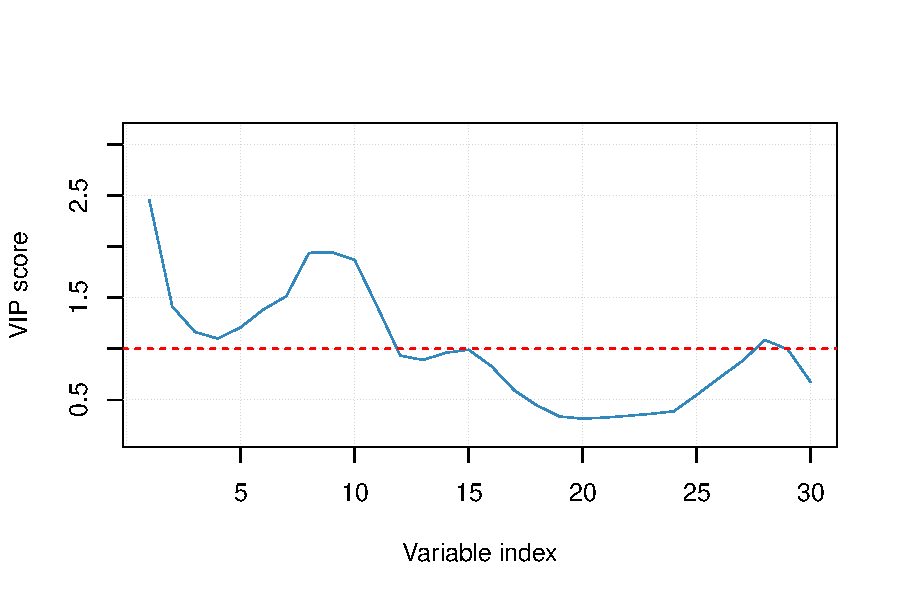
\includegraphics[width=0.65\textwidth]{figura41.pdf}
\caption[Plot of the VIP scores from the different variables in a PLS model]{Plot of the VIP scores from the different variables in a PLS model. The dashed red line marks the VIP=1 threshold.}
\label{figura41}
\end{figure}

\section{Selectivity Ratio}
In the majority of cases, several components are needed to adequately fit a model for a specific response \textbf{y}. By using the \textbf{y} vector as a target, it is possible to transform the PLS components to obtain a single predictive target-projected component, which is analogous to the predictive component in orthogonal partial least squares \parencite{bylesjo2006opls}. The selectivity ratio (SR) is estimated by calculating the ratio between explained and residual variance of the variables on that target-projected component \parencite{rajalahti2009biomarker}. Briefly, by selecting the normalized regression coefficients as PLS weights

\begin{equation}
\textbf{\text{w}}_{TP}=\textbf{\text{b}}_{PLS}/\|\textbf{\text{b}}_{PLS}\|
\label{equation30}
\end{equation}

and calculating target-projected scores by projection on the matrix of variables

\begin{equation}
\textbf{\text{t}}_{TP}=\textbf{\text{Xw}}_{TP}=\textbf{\text{Xb}}_{PLS}/\|\textbf{\text{b}}_{PLS}\|=\hat{\textbf{\text{y}}}/\|\textbf{\text{b}}_{PLS}\|
\label{equation31}
\end{equation}

it is showed that the target-projected scores are proportional to the vector of predicted responses.

The target-projected loadings can be calculated as

\begin{equation}
\textbf{\text{p}}^T_{TP}=\textbf{\text{t}}^T_{TP}\textbf{\text{X}}/(\textbf{\text{t}}^T_{TP}\textbf{\text{t}}_TP)=\textbf{\text{b}}^T_{PLS}/\|\textbf{\text{b}}_{PLS}\|*(\textbf{\text{X}}^T\textbf{\text{X}})/\|\textbf{\text{t}}_{TP}\|^2
\label{equation32}
\end{equation}

This shows that the target-projected loadings are the product of the normalized regression coefficients and the covariance matrix of the variables scaled by the inverse of the variance of the target-projected scores. So the target-projected loading vector combines the predictive ability of a variable with its explanatory power.

The target projection model can then be expressed as

\begin{equation}
\textbf{\text{X}}=\textbf{\text{X}}_{TP}+\textbf{\text{E}}_{TP}=\textbf{\text{t}}_{TP}\textbf{\text{p}}^T_{TP}+\textbf{\text{E}}_{TP}
\label{equation33}
\end{equation}

From here, explained and residual variance ($v_{expl,j}$ and $v_{res,j}$ can be computed for each variable $j$. Then the selectivity ratio is obtained by dividing explained and residual variance as follows

\begin{equation}
SR_j=v_{expl,j}/v_{res,j}, \ j=1,2,3 \dots
\label{equation34}
\end{equation}

As with the case of VIP scores and any other ranking method, the limit or threshold of SR value for considering a variable as relevant is arbitrary. Nevertheless, the authors of the original paper considered a 75\% of explained variance, corresponding to a SR of three, a reasonable threshold for selecting variables as relevant in predicting \textbf{y}.

An example of the SR computation results on the same PLS analysis presented in \autoref{figura41} for VIP scores is provided in \autoref{figura42}. It can be seen that conclusions from this method regarding relevant variables are coincident with those obtained using the VIP scores methods, so there is good agreement between both methods. There is only a slight disagreement regarding the first three variables, which are selected by the VIP scores methods and discarded by the selectivity ratio when using the standard threshold values for both methods.

\begin{figure}[hbtp]
\centering
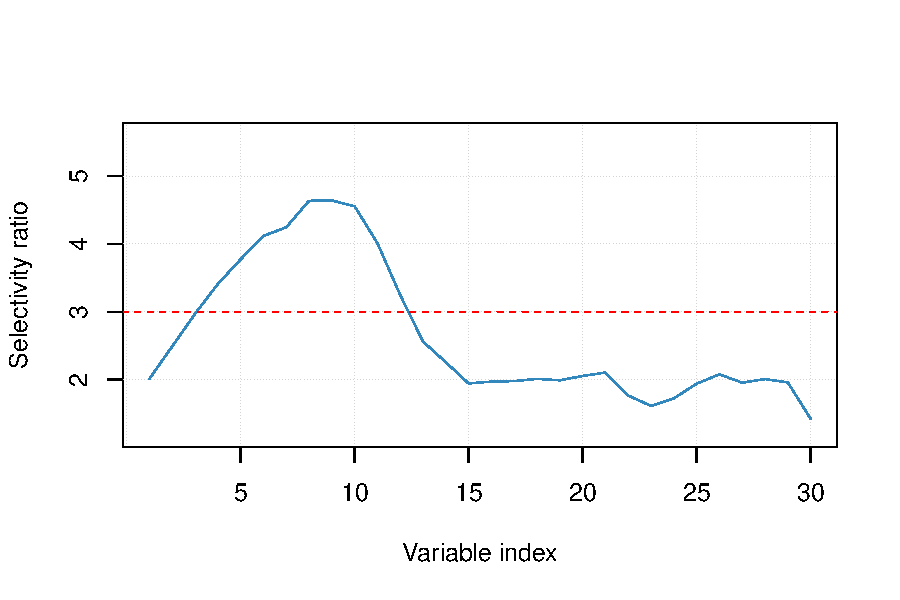
\includegraphics[width=0.65\textwidth]{figura42.pdf}
\caption[Plot of the SR from the different variables in a PLS model]{Plot of the SR from the different variables in a PLS model. The dashed red line marks the SR=3 threshold.}
\label{figura42}
\end{figure}

As of today. there are no published studies comparing the use of both methods in a comprehensive set of different data sets for the three-way case. However, a study of \textcite{farres2015comparison} compared both methods regarding variable selection performance and prediction capability in different two-way data sets. This study concluded that, for most data sets, the SR method selected fewer variables than the VIP method. In many cases, some of the variables selected by the VIP method were false positive candidates and some of the variables not selected by the SR were false negative candidates. Regarding prediction accuracy, each method was better that the other in a similar number of data sets, so final decision about the best of the two approaches should be based on the aims of the specific study being performed.

\section{Variable selection through L1 penalization}
As explained in \autoref{chapter:modern_techniques}, lasso applies a bias to the model fitting step of a linear or generalized linear model by shrinking all the coefficients using L1-penalization. This shrinkage reduces the complexity of the model, reducing variance and forcing some of the coefficients to be exactly zero, effectively performing variable selection at the same time as it increases predictive capacity reducing prediction error. Unfortunately the application of lasso, or its generalization elastic net, to three-way or multi-way data is not straightforward. The only approximations of these techniques for dealing with three-way data have been based on unfolding of the \textbf{\underline{X}} array \parencite{chiu2013multiway}. 

In \autoref{chapter:threeways}, the standard $N$-PLS algorithm has been presented as an appealing technique for modelling three- or multi-way data sets when there is a response to be predicted. However, in this chapter it has been exposed that, although there are some post modelling methods for estimating variable importance such as VIP \parencite{favilla2013assessing} and selectivity ratio \parencite{rajalahti2009biomarker},  it does not perform in-model variable selection, which would greatly increase its utility for analyzing metabolomic data sets. A suitable approach, recently published in \parencite{hervas2018sparse}, would consist in applying the L1 penalization from lasso inside the $N$-PLS algorithm to be able to perform variable selection at the model-fitting step while maintaining the capability of $N$-PLS of dealing with multi-way arrays. 

For this, it is proposed to use the soft-thresholding operator which can be derived from the lasso problem as follows:
\vspace{15pt}
\begin{enumerate}
    \item Assuming \textbf{X} (matrizied version of \textbf{\underline{X}}) is composed of orthogonal columns, the least squares solution is
    
    \begin{equation}
        \hat{\beta}^{LS}=(X^TX)^{-1}X^Ty=X^Ty
    \end{equation}
    \item Using the Lagrangian form, an equivalent problem to that considered would be
    
    \begin{equation}
        \min_\beta\frac{1}{2}||y-X\beta||^2_2+\lambda||\beta||_1
    \end{equation}
    \item Expansion of the first term gives
    
    \begin{equation}
        \frac{1}{2}y^Ty-y^TX\beta+\frac{1}{2}\beta^T\beta
    \end{equation}
    Since $y^Ty$ does not contain any of the variables of interest, it can be discarded, and one can consider the following equivalent problem
    
    \begin{equation}
        \min_\beta(-y^TX\beta+\frac{1}{2}||\beta||_2)+\lambda||\beta||_1
    \end{equation}
    Which can be rewritten as
    
    \begin{equation}
        \min_\beta \sum_{j=1}^{p}-\hat{\beta}^{LS}_j\beta_j+\frac{1}{2}\beta^2_j+\lambda|\beta_j|
    \end{equation}
    So, there is a sum of objectives as the objective function. Since each of them corresponds to a separate $\beta_j$, this means that each variable may be solved individually.
    \item For a certain $j$, the aim is to minimize
    
    \begin{equation}
        \mathcal{L}_j = -\hat{\beta}^{LS}_j\beta_j+\frac{1}{2}\beta^2_j+\lambda|\beta_j|
    \end{equation}
    If $\hat{\beta}^{LS}_j > 0$, then $\beta_j \geq 0$, otherwise one could just change its sign and get a lower value for the objective function. Correspondingly, if $\hat{\beta}^{LS}_j < 0$, then $\beta_j \leq 0$
    \item In the first case, if $\hat{\beta}^{LS}_j > 0$ and $\beta_j \geq 0$, then
    
    \begin{equation}
        \mathcal{L}_j = -\hat{\beta}^{LS}_j\beta_j+\frac{1}{2}\beta^2_j+\lambda\beta_j
    \end{equation}
    After differentiating respect to $\beta_j$ amd setting equal to zero, the result is $\beta_j = \hat{\beta}^{LS}_j-\lambda$. Since $\beta_j \geq 0$, the right-hand side must be non-negative, so the solution would be
    
    \begin{equation}
        \beta_j^{lasso}=sgn(\beta_j^{LS})(|\beta_j^{LS}|-\lambda)^+
    \end{equation}
    Which is the soft-thresholding operator.
    \item In the other case, if $\hat{\beta}^{LS}_j < 0$ and $\beta_j \leq 0$, then
    
    \begin{equation}
        \mathcal{L}_j = -\hat{\beta}^{LS}_j\beta_j+\frac{1}{2}\beta^2_j-\lambda\beta_j
    \end{equation}
    After differentiating respect to $\beta_j$ and setting equal to zero the result is $\beta_j = \hat{\beta}^{LS}_j+\lambda$. Since it is needed that $\beta_j \leq 0$ the solution is
    
    \begin{equation}
        \beta_j^{lasso}=sgn(\beta_j^{LS})(|\beta_j^{LS}|-\lambda)^+
    \end{equation}
    Which, again, gives the soft-thresholding operator.
\end{enumerate}

\vspace{20pt}
The soft-thresholding operator is well known in signal processing and image analysis, since it is used as a denoising filter in noisy images to obtain an approximation of the original image which gives the minimum mean square error \parencite{khare2005soft, joy2013denoising}. To understand how it works, the soft-thresholding function for a threshold of 3 has been represented in \autoref{figura28}. Its use to create sparsity in projection methods was first introduced by \textcite{zou2006sparse} in sparse Principal Component Analysis.
\vspace{10pt}

\begin{figure}[hbtp]
\centering
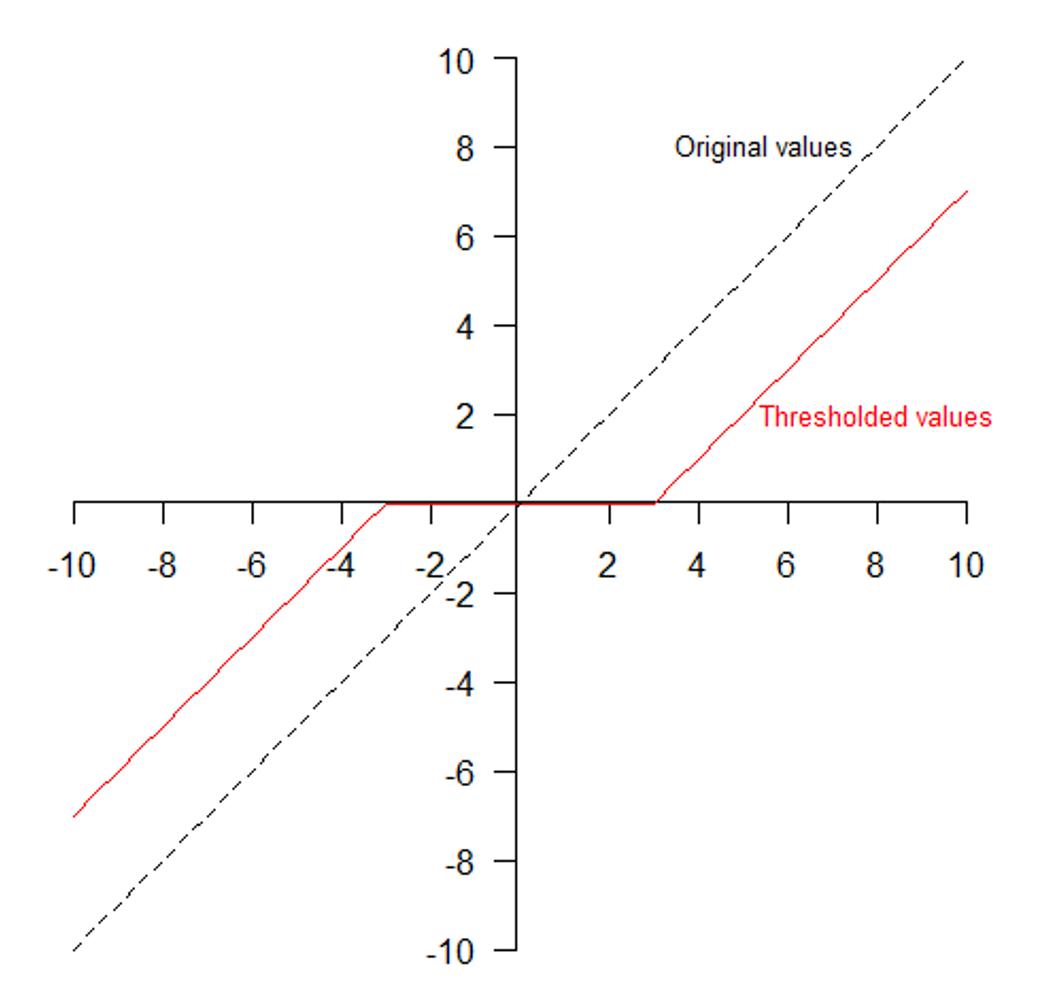
\includegraphics[width=0.6\textwidth]{figura28.png}
\caption[Soft-thresholding function]{Soft-thresholding function in the range x = [-10, 10] with a threshold $\lambda$ of 3. Values with $|x|$ higher than $\lambda$ have the threshold value substracted and values with $|x|$ equal or less than $\lambda$ are set to zero. Black dashed line represents the original values and red line represents the thresholded values.}
\label{figura28}
\end{figure}